\documentclass[11pt]{article}
\usepackage{graphicx}
\usepackage{hyperref}
\usepackage{geometry}
\geometry{margin=1in}

\title{Predicting Auto Insurance Claim Likelihood using Ensemble Learning under Extreme Class Imbalance}
\author{Sukaina D. Alkhalidy \\ Michigan State University \\ \texttt{alkhali5@msu.edu}}
\date{October 2025 \\ \url{https://github.com/sukaina13/cmse492_project}}

\begin{document}
\maketitle

\section*{Abstract}
This project investigates predicting whether an auto insurance policyholder will file a claim within the next year using the Porto Seguro Safe Driver dataset. The dataset is highly imbalanced, with only about 3.6\% of cases corresponding to claims. To handle this imbalance, ensemble learning methods such as the Balanced Random Forest and EasyEnsembleClassifier are applied and compared to simpler baselines like a majority-class model and logistic regression. Preliminary results show that the EasyEnsemble model improves recall for the minority class from 0.00 to approximately 0.58 and achieves an AUC of 0.63, indicating that ensemble-based resampling can significantly enhance risk prediction performance. The project aims to develop interpretable models that help insurers assess risk more fairly and efficiently.

\section{Background and Motivation}
Insurance providers face significant financial risk due to uncertainty in claim prediction. Accurately modeling the probability of a policyholder filing a claim enables better premium pricing and resource allocation. Traditional models such as logistic regression are limited by their sensitivity to class imbalance, leading to poor recall for rare claim events. Ensemble learning methods, especially balanced bagging and boosting approaches, offer robustness by resampling the minority data and aggregating decision trees. This project explores these methods to improve predictive reliability and interpretability for insurance claim prediction.

\section{Data Description}
The dataset originates from Porto Seguro, a Brazilian insurance company, and was released through a Kaggle competition. It includes 595,212 training samples and 58 predictive features capturing driver demographics, vehicle characteristics, and regional attributes. About 3.6\% of policyholders filed claims, resulting in an extreme class imbalance ratio of roughly 26:1. Missing data primarily occurs in a few categorical variables, while most features are complete and numeric.
\begin{figure}[h]
    \centering
    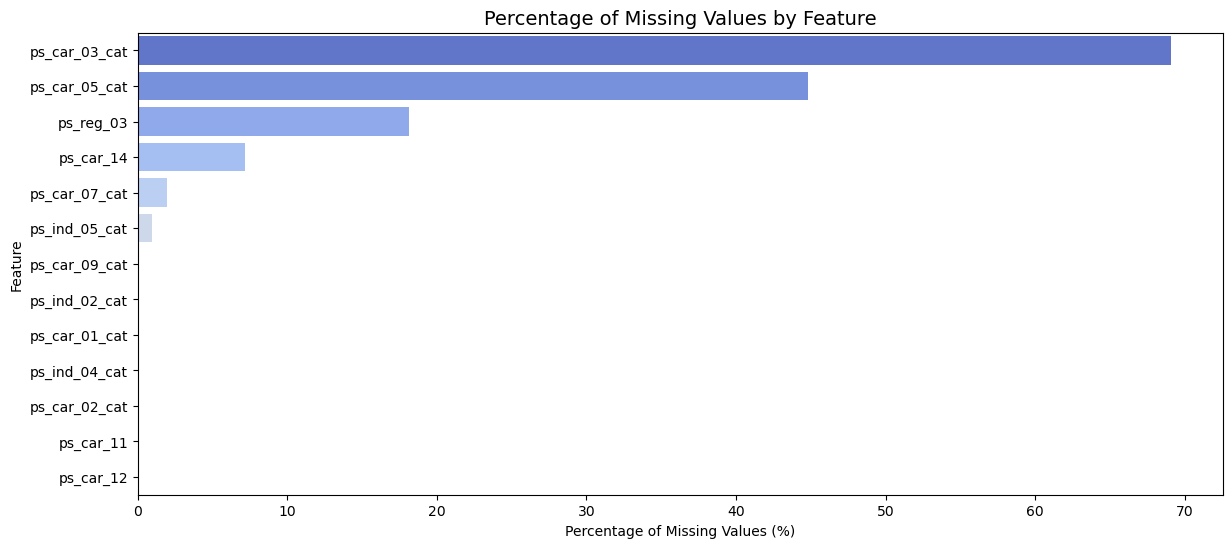
\includegraphics[width=0.8\textwidth]{../figures/missing_barplot.png}
    \caption{Percentage of missing values across major features.}
\end{figure}

\begin{figure}[h]
    \centering
    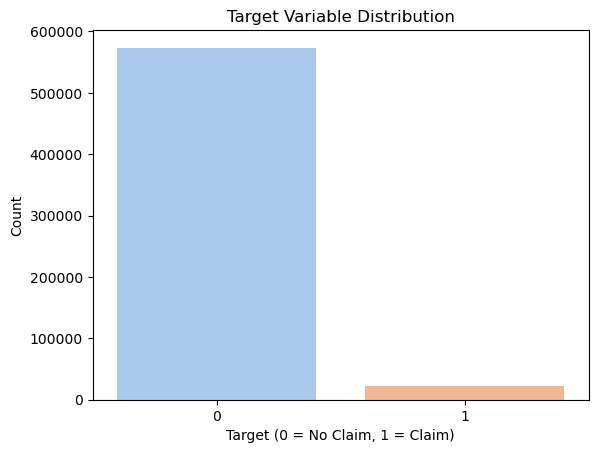
\includegraphics[width=0.8\textwidth]{../figures/target_distribution.png}
    \caption{Target variable distribution showing 96.4\% no-claim and 3.6\% claim cases.}
\end{figure}

Planned preprocessing includes imputing missing values with median/mode, dropping columns with over 50\% missingness, and using label encoding for categorical variables. Since tree-based methods are insensitive to scaling, normalization is not required.

\section{Proposed Methodology}
Three models of increasing complexity are compared:
\begin{enumerate}
    \item \textbf{Majority Class Baseline:} Always predicts no claim.
    \item \textbf{Logistic Regression:} Incorporates class weighting to account for imbalance.
    \item \textbf{Ensemble Models:} Balanced Random Forest and EasyEnsembleClassifier, both of which combine resampling with tree-based learners.
\end{enumerate}
\begin{figure}[h]
    \centering
    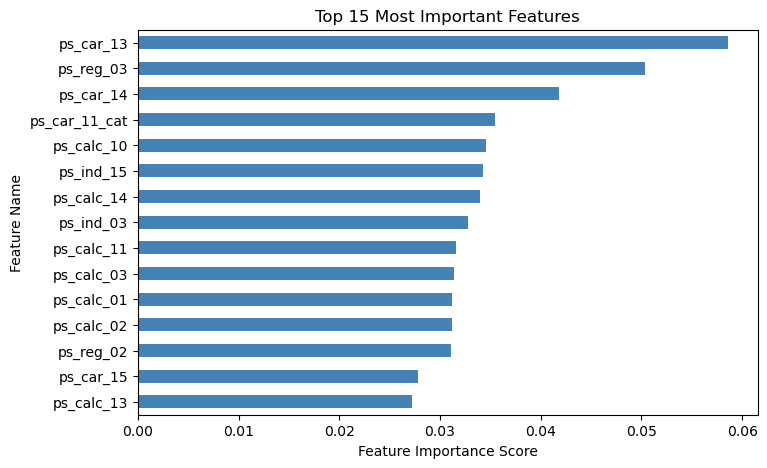
\includegraphics[width=0.8\textwidth]{../figures/feature_importance_balanced_rf.png}
    \caption{Top 15 most important features identified by Balanced Random Forest.}
\end{figure}
Model interpretability is enhanced through feature importance plots, while hyperparameter tuning via RandomizedSearchCV ensures optimal performance. EasyEnsemble is expected to outperform due to its adaptive boosting strategy over balanced subsets.

\section{Evaluation Framework}
Performance will be evaluated using precision, recall, F1-score, and area under the ROC curve (AUC). A stratified 70/15/15 train-validation-test split preserves class ratios. The baseline majority model serves as a reference point with 96.4\% accuracy but zero recall. Success will be defined as achieving recall above 0.55 and AUC above 0.65 for the minority class, improving both detection and ranking ability for true claim cases.

\section{Timeline and Milestones}
\begin{itemize}
    \item \textbf{Week 9 (Oct 28–Nov 3):} Complete exploratory data analysis and baseline models.
    \item \textbf{Week 10–11:} Implement ensemble models and conduct hyperparameter tuning.
    \item \textbf{Week 12:} Evaluate results and refine interpretability analysis.
    \item \textbf{Week 13–14:} Draft final report and prepare presentation.
    \item \textbf{Week 15 (Dec 2–8):} Final presentation and submission.
\end{itemize}

\begin{figure}[h]
    \centering
    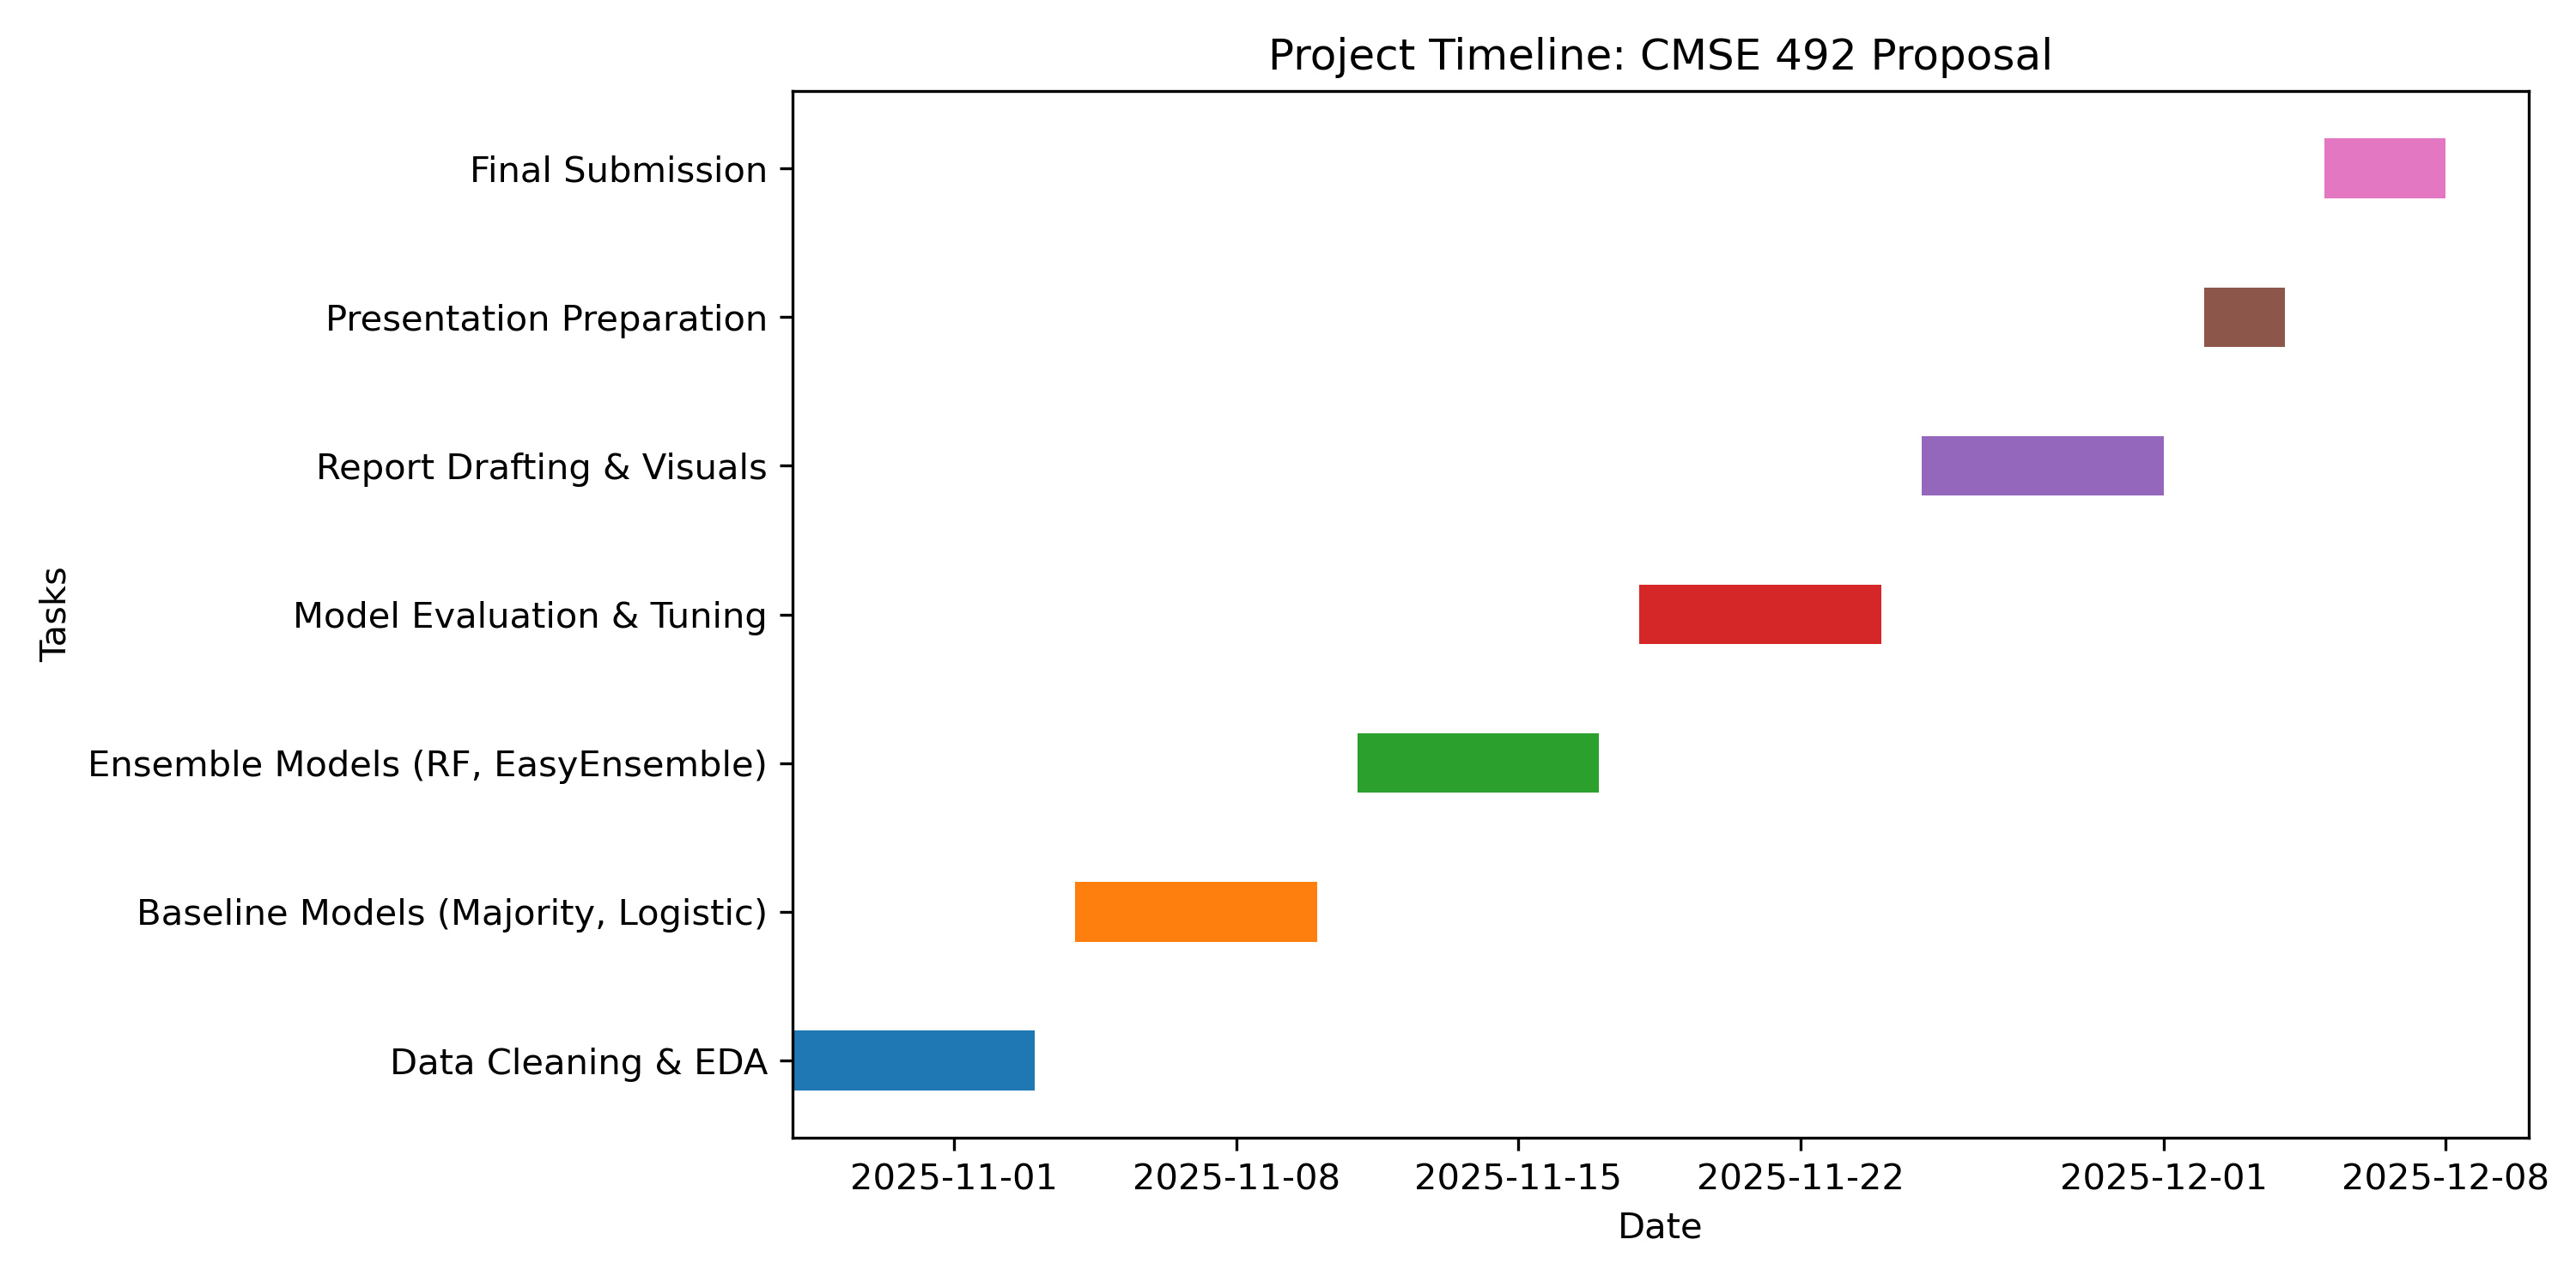
\includegraphics[width=0.9\textwidth]{../figures/gantt_chart.png}
    \caption{Planned Gantt chart outlining project tasks and milestones.}
\end{figure}

\end{document}
